\chapter{TINJAUAN PUSTAKA}
\label{chap:tinjauanpustaka}

% Ubah bagian-bagian berikut dengan isi dari tinjauan pustaka
% Demi mendukung penelitian ini, \lipsum[1][1-5]

\section{Hasil Penelitian Terdahulu}
\label{sec:hasilpenelitianterdahulu}
Penelitian ini mengambil referensi dari beberapa penelitian terdahulu dengan topik yang sama ataupun beririsan, serta dasar pengembangan dan inovasi yang akan pada penelitian ini. Berikut adalah beberapa penelitian terdahulu yang diambil sebagai referensi:

\subsection{Deteksi Kendaraan Truk pada Video Menggunakan Metode Tiny-YOLOv4}
\label{subsec:deteksikendaraantrukprismadika}
Penelitian oleh Prismadika Yuniar et al. \parencite*{prismadika2023} mengkaji deteksi truk secara \emph{real-time} dalam video pengamatan di jalan raya. Tantangan muncul karena truk memiliki dimensi serupa dengan bus dan struktur mekanis mirip pikap. Pada tahap awal, model YOLO asli hanya mampu mendeteksi bagian kepala dan bak truk tanpa memperhitungkan muatan. Oleh karena itu, dibuat \emph{custom dataset} dengan \emph{bounding box} untuk seluruh bagian truk beserta muatannya.

Tiny-YOLOv4 dipilih karena lebih ringan dan kompatibel dengan perangkat beragam. Pengujian pada tiga perangkat menunjukkan bahwa Laptop Acer E5 mencapai akurasi 98,2\% pada 13 FPS, Laptop Lenovo Legion 5 98\% pada 28 FPS, dan PC Dell Precision 3640 Tower 97,5\% pada 38 FPS. 

Hasil yang didapatkan yaitu FPS yang lebih tinggi cenderung menurunkan akurasi, dan perangkat dengan CPU di atas 3.0 GHz, RAM minimal 16 GB, dan GPU lebih dari 4 GB mampu menjalankan deteksi secara \emph{real-time} dengan baik.

\subsection{Sistem Deteksi Kendaraan \emph{Overdimension} secara \emph{Real-time} menggunakan \emph{Deep Learning} di Jalan Raya}
\label{subsec:deteksikendaraanoverdimensionhamayan}
Penelitian ini dilakukan oleh Ahmad Hamayan Nabih \parencite*{hamayan2024}. Penelitian ini bertujuan untuk mengembangkan sistem deteksi kendaraan overdimension secara \emph{real-time} menggunakan \emph{deep learning} di jalan raya. Sistem ini menggunakan model YOLOv8 yang telah dimodifikasi untuk mendeteksi kendaraan \emph{overdimension}. \emph{Dataset} yang digunakan adalah \emph{dataset} yang telah diambil dari jalan raya di Indonesia. Variasi yang digunakan yaitu variasi akurasi pada berbagai macam perangkat dan model YOLOv8.

Variasi perangkat meliputi PC dengan \emph{External VGA} NVIDIA GeForce GTX 1650Ti, Laptop tanpa \emph{External VGA}, dan Intel NUC i5 Gen 11. Hasil yang didapatkan yaitu PC dengan \emph{External VGA} NVIDIA GeForce GTX 1650Ti mampu mendeteksi kendaraan \emph{overdimension} dengan akurasi 85\% - 90\% pada 33 FPS - 63 FPS, Laptop tanpa \emph{External VGA} dengan akurasi 87\% - 92\% pada 7 FPS - 10 FPS, dan Intel NUC i5 Gen 11 dengan akurasi 79\% - 90\% pada 2 FPS. Sedangkan variasi model YOLOv8 meliputi YOLOv8n dan YOLOv8s, dimana YOLOv8n di-\emph{training} dengan 50 \emph{epoch} dan YOLOv8s di-\emph{training} dengan 75 \emph{epoch}.

Kesimpulan yang didapatkan yaitu model YOLOv8n lebih baik dari segi FPS dibandingkan dengan YOLOv8s namun memiliki akurasi yang lebih rendah. Sedangkan model pembandingnya, yaitu YOLOv8s memiliki akurasi yang lebih tinggi namun FPS yang lebih rendah. Kemudian juga ditemukan bahwa perangkat dengan spesifikasi yang lebih tinggi mampu mendeteksi kendaraan \emph{overdimension} dengan akurasi yang lebih tinggi dan FPS yang lebih tinggi.

\subsection{Implementasi Sistem Penghitung Kendaraan Otomatis Berbasis \emph{Computer Vision}}
\label{subsec:implementasisistemhitungkendaraan}
Penelitian ini dilakukan oleh Dolly Indra et al. \parencite*{dolly2023}. Penelitian ini bertujuan untuk mengembangkan sistem penghitung kendaraan otomatis di tempat pencucian kendaraan. Sistem ini menggunakan Raspberry Pi 4 sebagai \emph{edge device} dan model SSD MobileNet V2 sebagai model deteksi. Sistem ini mampu menghitung jumlah kendaraan yang masuk dan keluar dari tempat pencucian kendaraan secara \emph{real-time} yang terhubung dengan aplikasi \emph{mobile}.

Hasil yang didapatkan yaitu sistem otomatis mampu mendeteksi kendaraan mobil dan motor dengan rata-rata tingkat akurasi sebesar 46,6 \% dan aplikasi yang terdapat pada \emph{smartphone} mampu menghitung jumlah kendaraan yang masuk dan keluar dari tempat pencucian kendaraan.

\subsection{\emph{Fast Vehicle Detection Algorithm in Traffic Scene Based on Improved SSD}}
\label{subsec:fastvehicledetectionalgorithm}

Penelitian ini dilakukan oleh Zhichao Chen et al. \parencite*{Chen2022Fast} mengusulkan peningkatan pada algoritma Single Shot Multibox Detector (SSD) untuk deteksi kendaraan di lingkungan lalu lintas yang kompleks. Inovasi utama adalah penggunaan MobileNet v2 sebagai backbone, menggantikan VGG16 yang lebih berat secara komputasi. Selain itu, ditambahkan channel attention mechanism (SE module) untuk memperkuat fitur penting dan modul dekonvolusi untuk melakukan bottom–top feature fusion, sehingga informasi semantik pada fitur dangkal dapat diperbaiki.

Hasil eksperimen menunjukkan rata-rata presisi (AP) sebesar 82,59\% pada dataset publik BDD100K dan 84,83\% pada KITTI. Waktu inferensi per gambar hanya 73 ms, sekitar 5/11 dari waktu model SSD orisinal, sehingga terjadi peningkatan baik pada kecepatan maupun akurasi. Penelitian ini menegaskan bahwa kombinasi backbone ringan, mekanisme atensi, dan fusi fitur dapat menghasilkan deteksi kendaraan yang efisien dan akurat, sangat relevan untuk aplikasi \emph{real-time} dan perangkat dengan sumber daya terbatas

\subsection{\emph{Edge Intelligence Empowered Vehicle Detection and Image Segmentation for Autonomous Vehicles}}
\label{subsec:edgeintelligenceempoweredvehicledetection}

Penelitian ini dilakukan oleh Zhinchao Chen et al. \parencite*{Chen2023Edge}mengembangkan pendekatan \emph{edge intelligence} untuk deteksi kendaraan dan segmentasi citra pada sistem transportasi cerdas dan kendaraan otonom. \emph{Edge intelligence} menggabungkan kecerdasan buatan dan \emph{edge computing} untuk memproses data secara lokal di dekat sumber data, sehingga mengurangi latensi, menghemat sumber daya transmisi, meningkatkan keamanan data, dan mengoptimalkan pemanfaatan sumber daya antara perangkat, edge, dan cloud.

Inovasi utama dari penelitian ini adalah deteksi kendaraan berbasis improved YOLOv4 dimana Peneliti mengintegrasikan \emph{Efficient Channel Attention} (ECA) ke dalam modul konvolusi YOLOv4 dan menambahkan \emph{High-Resolution Network} (HRNet) untuk meningkatkan kemampuan deteksi kendaraan, khususnya pada edge device yang memiliki keterbatasan sumber daya komputasi. Kemudian juga segmentasi citra berbasis improved DeepLabv3+ dimana peneliti Model DeepLabv3+ dimodifikasi dengan mengganti backbone menjadi MobileNetV2 dan menggunakan metode \emph{softpool} untuk mengurangi kehilangan informasi saat segmentasi, sehingga ukuran jaringan lebih kecil dan akurasi segmentasi meningkat.

Hasil dari penelitian ini yaitu:
\begin{itemize}[nolistsep]
  \item Akurasi deteksi kendaraan meningkat dari 82,03\% menjadi 86,22\% (Average Precision/AP).
  \item Akurasi segmentasi citra (mean Intersection over Union/mIoU) naik dari 73,32\% menjadi 75,63\%.
\end{itemize}
Model yang diusulkan dapat berjalan efisien pada edge device, mendukung kebutuhan \emph{real-time} dan penghematan bandwidth.

\section{Teori/Konsep Dasar}
\label{sec:teorikonsepdasar}
 Berikut adalah teori atau konsep dasar sebagai landasan teoritis dalam pelaksanaan penelitian ini.
 
\subsection{Regulasi Pemerintah tentang Kendaraan \emph{Overdimension}}

Kendaraan \emph{overdimension} adalah kendaraan yang memiliki dimensi melebihi ketentuan yang ditetapkan oleh pemerintah. Pemerintah Indonesia telah mengatur ketentuan mengenai kendaraan \emph{overdimension} dalam Peraturan Pemerintah Nomor 55 Tahun 2012 Pasal 54 dan 55 tentang Ukuran Kendaraan Bermotor \parencite*{ppno55thn2012}. Berikut adalah ketentuan yang diatur dalam peraturan tersebut:

\subsubsection{Peraturan Pemerintah Nomor 55 Tahun 2012 Pasal 54}

\begin{enumerate}[nolistsep]
  \item Panjang tidak melebihi:
  \begin{enumerate}[nolistsep]
    \item 12.000 (dua belas ribu) milimeter untuk Kendaran Bermotor tanpa Kereta Gandengan atau Kereta Tempelan selain Mobil Bus;
    \item 13.500 (tiga belas ribu lima ratus) milimeter untuk Mobil Bus tunggal;
    \item 18.000 (delapan belas ribu) milimeter untuk Kendaraan Bermotor yang dilengkapi dengan Kereta Gandengan atau Kereta Tempelan.
  \end{enumerate}
  \item Lebar tidak melebihi 2.500 (dua ribu lima ratus)
  milimeter;
  \item Tinggi tidak melebihi 4.200 (empat ribu dua ratus) milimeter dan tidak lebih dari 1,7 (satu koma tujuh) kali lebar Kendaraan;
  \item Sudut pergi Kendaraan paling sedikit 8° (delapan derajat) diukur dari atas permukaan bidang atau jalan yang datar; dan
  \item Jarak bebas antara bagian permanen paling bawah Kendaraan Bermotor terhadap permukaan bidang jalan tidak bersentuhan dengan permukaan bidang jalan.
  \item Panjang bagian Kendaraan yang menjulur ke belakang dari sumbu paling belakang maksimum 62,50\% (enam puluh dua koma lima nol persen) dari jarak sumbunya, sedangkan yang menjulur ke depan dari sumbu paling depan maksimum 47,50\% (empat puluh tujuh koma lima nol persen) dari jarak sumbunya.
  \item Dalam hal Kendaraan Bermotor memiliki tinggi keseluruhan lebih dari 3.500 (tiga ribu lima ratus) milimeter, wajib dilengkapi dengan tanda.
  \item Tanda sebagaimana dimaksud pada nomor 7 berupa tulisan yang mudah dilihat oleh pengemudi di dalam ruang pengemudi.
\end{enumerate}

\subsubsection{Peraturan Pemerintah Nomor 55 Tahun 2012 Pasal 55}

\begin{enumerate}[nolistsep]
  \item Ukuran bak muatan Mobil Barang disesuaikan dengan konfigurasi sumbu, JBB, JBI, dan spesifikasi tipe landasan Kendaraan Bermotor.
  \item Bak muatan Mobil Barang sebagaimana dimaksud pada ayat (1) terdiri atas:
  \begin{enumerate}[nolistsep]
    \item bak muatan terbuka; dan
    \item bak muatan tertutup. 
  \end{enumerate}
  \item Bak muatan terbuka dan tertutup sebagaimana dimaksud pada ayat (2) harus memenuhi persyaratan paling sedikit:
  \begin{enumerate}[nolistsep]
    \item panjang, lebar, dan tinggi ukuran bak muatan harus sesuai dengan spesifikasi teknis Kendaraan Bermotor dan daya angkut;
    \item jarak antara dinding terluar bagian belakang kabin dengan bak muatan bagian depan paling sedikit 150 (seratus lima puluh) milimeter untuk kendaraan sumbu belakang tunggal dan 200 (dua ratus) milimeter untuk Kendaraan Bermotor dengan sumbu belakang ganda atau lebih;
    \item dinding terluar bak muatan bagian belakang tidak melebihi ujung landasan bagian belakang kecuali untuk dump truck; dan
    \item lebar maksimum bak muatan terbuka tidak melebihi:
    \begin{enumerate}[nolistsep]
      \item 50 (lima puluh) milimeter dari ban terluar pada sumbu kedua atau sumbu belakang Kendaraan untuk Kendaraan Bermotor sumbu ganda; atau
      \item lebar kabin ditambah 50 (lima puluh) milimeter pada sisi kiri dan 50 (lima puluh) milimeter pada sisi kanan untuk Kendaraan Bermotor sumbu tunggal.
    \end{enumerate} 
  \end{enumerate}
  \item Dalam hal tinggi bak muatan terbuka pada Mobil Barang sebagaimana dimaksud pada ayat (2) huruf a lebih rendah dari jendela kabin belakang, pada jendela kabin belakang Mobil Barang harus dipasang teralis.
  \item Untuk bak muatan tertutup selain memenuhi persyaratan sebagaimana dimaksud pada ayat (3) harus memenuhi persyaratan tinggi bak muatan tertutup diukur dari permukaan tanah paling tinggi 4.200 (empat ribu dua ratus) milimeter dan tidak lebih dari 1,7 (satu koma tujuh) kali lebar Kendaraan Bermotor.
\end{enumerate}

Dari ketentuan tersebut, dilakukan pendekatan rumus untuk menghitung dimensi kendaraan \emph{overdimension} berdasarkan ketentuan yang diatur oleh pemerintah. Hal ini akan membantu dalam mengidentifikasi kendaraan yang melanggar batas dimensi yang diizinkan. Rumus yang digunakan adalah sebagai berikut:

\begin{itemize}[nolistsep]
  \item Panjang: \( L \leq 12000 \) mm
  \item Lebar: \( W \leq 2500 \) mm
  \item Tinggi: \( H \leq 4200 \) mm dan \( H \leq 1.7 \times W \)
  \item Sudut pergi: \( \theta \geq 8^\circ \)
  \item Jarak bebas: \( D \geq 0 \) mm
  \item Panjang bagian belakang: \( L_{\mathrm{belakang}} \leq 0.625 \times L \)
  \item Panjang bagian depan: \( L_{\mathrm{depan}} \leq 0.475 \times L \)
  \item Tinggi keseluruhan: \( H_{\mathrm{keseluruhan}} > 3500 \) mm
  \item Lebar bak muatan terbuka: \( W_{\mathrm{bak}} \leq 50 \) mm
  \item Tinggi bak muatan tertutup: \( H_{\mathrm{bak}} \leq 4200 \) mm dan \( H_{\mathrm{bak}} \leq 1.7 \times W \)
  \item Jarak antara dinding terluar: \( D_{\mathrm{terluar}} \geq 150 \) mm
  \item Lebar bak muatan terbuka: \( W_{\mathrm{bak}} \leq 50 \) mm
\end{itemize}

Namun dalam penelitian ini, rumus tersebut tidak digunakan secara langsung. Sebagai gantinya, akan digunakan model \emph{deep learning} untuk mengidentifikasi kendaraan \emph{overdimension} berdasarkan karakteristik visualnya. Hal ini akan memungkinkan sistem untuk melakukan deteksi secara otomatis dan \emph{real-time} tanpa memerlukan perhitungan manual.

\subsection{Regulasi Gandar Kendaraan Bermotor}
\label{subsec:regulasigandar}

Gandar kendaraan bermotor merupakan komponen penting yang diatur secara ketat dalam regulasi pemerintah \parencite*{kemenhub2015}. Regulasi ini bertujuan untuk menjamin keselamatan, melindungi infrastruktur jalan, dan mengoptimalkan efisiensi transportasi. Pengaturan gandar mencakup berbagai aspek teknis dan operasional yang harus dipatuhi oleh setiap kendaraan bermotor yang beroperasi di jalan raya Indonesia.

\subsubsection{Konsep Dasar Gandar}
Gandar, atau dalam bahasa Inggris disebut axle, adalah komponen struktural utama pada kendaraan yang memiliki fungsi ganda. Pertama, sebagai poros penopang roda yang mentransmisikan beban vertikal dari berat kendaraan dan muatan ke permukaan jalan. Kedua, sebagai penghubung mekanis dengan sasis kendaraan yang menyalurkan gaya-gaya dinamis selama kendaraan bergerak \parencite*{cebon1989assessment}.

Berdasarkan fungsinya, gandar dapat diklasifikasikan menjadi dua jenis utama:
\begin{itemize}[nolistsep]
  \item \textbf{Gandar Penggerak (Drive Axle):} Gandar yang terhubung dengan sistem transmisi dan menerima tenaga dari mesin untuk menggerakkan kendaraan. Gandar ini biasanya dilengkapi dengan diferensial untuk mengakomodasi perbedaan kecepatan roda saat berbelok.
  \item \textbf{Gandar Bebas (Dead/Idler Axle):} Gandar yang hanya berfungsi sebagai penopang beban dan tidak terhubung dengan sistem penggerak. Gandar ini umumnya ditemukan pada bagian depan kendaraan atau sebagai gandar tambahan pada kendaraan berat.
\end{itemize}

Konfigurasi sumbu pada kendaraan bermotor diatur dalam PP No. 55 Tahun 2012 \parencite*{ppno55thn2012}, yang mengklasifikasikan beberapa tipe standar:
\begin{itemize}[nolistsep]
  \item \textbf{Konfigurasi 1.1:} Dua sumbu tunggal, umum pada kendaraan ringan
  \item \textbf{Konfigurasi 1.2:} Satu sumbu tunggal di depan dan satu sumbu ganda di belakang, tipikal pada truk sedang
  \item \textbf{Konfigurasi 1.22:} Satu sumbu tunggal di depan dan dua sumbu ganda di belakang, umumnya pada truk berat
\end{itemize}

\subsubsection{Beban dan Muatan}
Regulasi beban dan muatan kendaraan didasarkan pada tiga parameter utama yang saling terkait \parencite*{kemenhub2015}:

\begin{itemize}[nolistsep]
  \item \textbf{Beban Gandar:} Merupakan total berat yang ditanggung oleh satu gandar, yang terdiri dari:
  \begin{itemize}[nolistsep]
    \item Berat kosong kendaraan yang terdistribusi ke gandar tersebut
    \item Berat muatan yang ditopang oleh gandar
    \item Berat komponen pendukung seperti suspensi dan roda
  \end{itemize}
  
  \item \textbf{Muatan Sumbu Terberat (MST):} Parameter kritis yang menentukan batas beban maksimum yang diizinkan untuk setiap sumbu atau kelompok sumbu \parencite*{ppno55thn2012}. MST ditetapkan berdasarkan:
  \begin{itemize}[nolistsep]
    \item Kapasitas desain gandar
    \item Daya dukung jalan
    \item Faktor keselamatan
  \end{itemize}
  
  \item \textbf{Jumlah Berat yang Diizinkan (JBI):} Total berat maksimum kendaraan beserta muatannya yang diizinkan beroperasi di jalan. JBI mempertimbangkan:
  \begin{itemize}[nolistsep]
    \item Distribusi beban antar sumbu
    \item Kapasitas komponen kendaraan
    \item Batasan regulasi yang berlaku
  \end{itemize}
\end{itemize}

\subsubsection{Dampak Beban Berlebih}
Pelanggaran terhadap batas beban yang ditetapkan dapat menyebabkan berbagai dampak negatif pada infrastruktur jalan dan keselamatan. Menurut studi yang dilakukan oleh Huang \parencite*{huang2004pavement}, beban gandar berlebih dapat mengakibatkan:

\begin{itemize}[nolistsep]
  \item \textbf{Kerusakan Infrastruktur:} Manifestasi kerusakan meliputi:
  \begin{itemize}[nolistsep]
    \item \emph{Fatigue Cracking} (retak fatik): Retakan yang terbentuk akibat beban berulang yang melebihi kapasitas struktur perkerasan
    \item \emph{Rutting} (deformasi permanen): Cekungan yang terbentuk pada jalur roda akibat deformasi plastis material perkerasan
    \item \emph{Ravelling} (lepasnya butiran): Terlepasnya material permukaan jalan akibat hilangnya daya ikat antar agregat
  \end{itemize}
  
  \item \textbf{Hukum Pangkat Empat:} Prinsip fundamental dalam analisis kerusakan jalan yang menyatakan bahwa tingkat kerusakan meningkat secara eksponensial (pangkat empat) terhadap peningkatan beban gandar. Secara matematis dapat dinyatakan:
  \begin{equation}
    \mbox{Faktor Kerusakan} = \left(\frac{\mbox{Beban Aktual}}{\mbox{Beban Standar}}\right)^4
  \end{equation}
  
  Sebagai contoh, jika beban gandar meningkat 20\% dari standar:
  \begin{equation}
    \mbox{Faktor Kerusakan} = (1.20)^4 = 2.07
  \end{equation}
  
  Artinya, peningkatan beban sebesar 20\% akan menyebabkan kerusakan lebih dari dua kali lipat dari kondisi normal.
\end{itemize}

\subsubsection{Persyaratan Teknis dan Pengujian}
Untuk memastikan kepatuhan terhadap regulasi dan menjamin keselamatan, kendaraan bermotor harus melalui serangkaian pengujian dan pemeriksaan \parencite*{ditjenhubdat2021}:

\begin{itemize}[nolistsep]
  \item \textbf{Kelaikan Jalan:} Evaluasi menyeluruh yang mencakup:
  \begin{itemize}[nolistsep]
    \item Kondisi fisik gandar dan komponen pendukungnya
    \item Sistem suspensi dan karakteristik redamannya
    \item Efektivitas sistem pengereman pada setiap gandar
    \item Keseimbangan distribusi beban antar gandar
  \end{itemize}
  
  \item \textbf{Uji Tipe:} Serangkaian pengujian komprehensif terhadap prototipe kendaraan \parencite*{kemenhub2016} yang meliputi:
  \begin{itemize}[nolistsep]
    \item Pengujian kekuatan struktur gandar
    \item Verifikasi kapasitas beban sesuai desain
    \item Evaluasi kinerja sistem pengereman
    \item Pengujian stabilitas kendaraan
  \end{itemize}
  
  \item \textbf{Uji Berkala:} Pemeriksaan rutin yang dilakukan untuk memastikan:
  \begin{itemize}[nolistsep]
    \item Tidak ada deformasi atau kerusakan pada gandar
    \item Sistem suspensi berfungsi optimal
    \item Distribusi pengereman sesuai standar
    \item Kesesuaian dengan batas beban yang diizinkan
  \end{itemize}
\end{itemize}

Pemahaman mendalam tentang regulasi gandar ini penting dalam pengembangan sistem deteksi kendaraan \emph{overdimension}, karena menjadi dasar dalam menentukan parameter dan batasan yang akan digunakan dalam algoritma deteksi. Meskipun penelitian ini menggunakan pendekatan visual melalui \emph{deep learning}, pengetahuan tentang aspek teknis dan regulasi gandar membantu dalam memahami karakteristik dan pola yang perlu diidentifikasi oleh sistem.

\subsection{\emph{Neural Network}}
\emph{Neural Network} (NN), atau jaringan saraf, adalah fondasi dari banyak model \emph{deep learning}, termasuk CNN. Bagian ini akan membahas konsep dasar NN mulai dari perceptron, fungsi aktivasi, mekanisme \emph{feed forward}, \emph{backpropagation}, \emph{loss function}, dan \emph{optimizer}.

\begin{figure}[H]
  \centering
  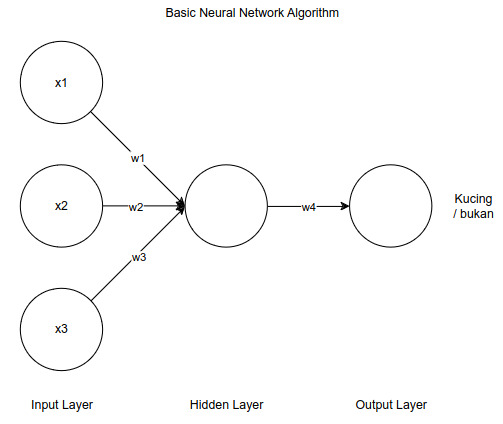
\includegraphics[scale=0.6]{gambar/bab2-basic-nn.jpeg}
  \caption{Diagram sederhana dari \emph{Neural Network}}
  \label{fig:basic_nn}
\end{figure}

\subsubsection{\emph{Perceptron}}
\emph{Perceptron} merupakan dasar dari NN, yang diperkenalkan oleh Frank Rosenblatt pada tahun 1958 \parencite*{rosenblatt1958perceptron}. \emph{Perceptron} adalah model jaringan saraf tiruan yang paling sederhana, yang memodelkan sebuah neuron dalam otak.

Struktur dasar \emph{perceptron} terdiri dari \emph{input} \( x_1, x_2, \dots, x_n \), \emph{weights} (bobot) \( w_1, w_2, \dots, w_n \), dan bias \( b \). \emph{Output} dari \emph{perceptron} dihitung menggunakan Persamaan \ref{eq:perceptron}:

\begin{equation}
  \label{eq:perceptron}
  y = f(w \cdot x + b)
\end{equation}

dimana \( f \) adalah fungsi aktivasi, \( w \cdot x \) adalah \emph{dot product} antara vektor bobot dan vektor input, dan \( b \) adalah bias.
 
 \subsubsection{\emph{Activation Function}}
 \emph{Activation function} menentukan \emph{output} dari sebuah \emph{neuron} berdasarkan \emph{input} total yang diterima. Beberapa fungsi aktivasi yang sering digunakan adalah:
 \begin{itemize}[nolistsep]
   \item Sigmoid: \( \sigma(x) = \frac{1}{1 + e^{-x}} \). Fungsi ini menghasilkan \emph{output} dalam rentang \( (0, 1) \), yang berguna untuk tugas klasifikasi biner.
   \item Tanh: \( \tanh(x) = \frac{e^{x} - e^{-x}}{e^{x} + e^{-x}} \). Fungsi ini menghasilkan \emph{output} dalam rentang \( (-1, 1) \), yang membantu dalam mengatasi masalah \emph{vanishing gradient}. Yaitu ketika nilai \emph{input} yang besar atau kecil menyebabkan gradien yang sangat kecil.
   \item ReLU (Rectified Linear Unit): \( ReLU(x) = \max(0, x) \). Fungsi ini menghasilkan \emph{output} \( 0 \) jika \emph{input} \( x \leq 0 \) dan \( x \) jika \( x > 0 \). ReLU adalah fungsi aktivasi yang paling umum digunakan dalam arsitektur NN modern karena sederhana dan efektif.
 \end{itemize}

  Gambar \ref{fig:sigmoid_function} (Sigmoid), \ref{fig:tanh_function} (Tanh), dan \ref{fig:relu_function} (ReLU) menunjukkan grafik dari \emph{activation function} yang disebutkan di atas.

  \begin{figure}[htbp]
    \centering
    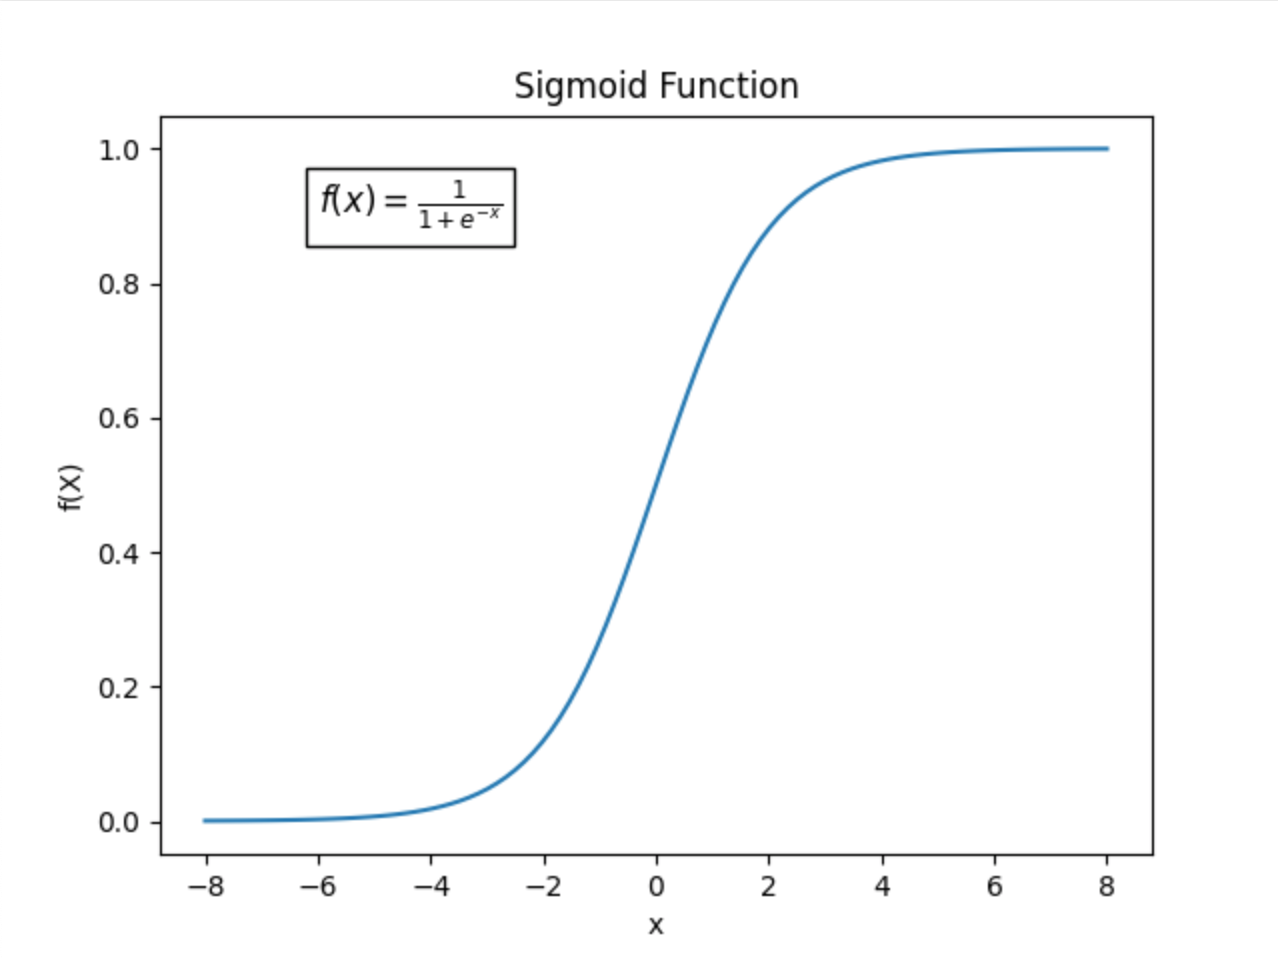
\includegraphics[scale=0.6]{gambar/bab2-grafik-sigmoid.png}
  \caption{Grafik \emph{Activation function Sigmoid}}
  \label{fig:sigmoid_function}
  \end{figure}

  \begin{figure}[htbp]
    \centering
    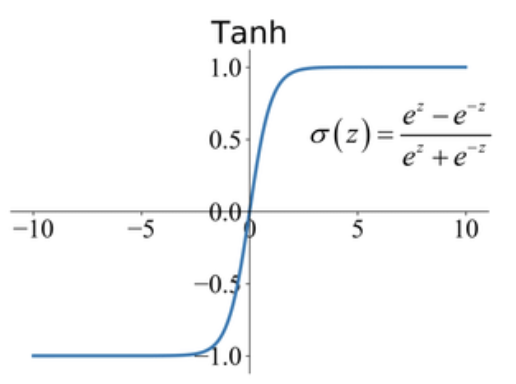
\includegraphics[scale=1]{gambar/bab2-grafik-tanh.png}
    \caption{Grafik \emph{Activation function Tanh}}
    \label{fig:tanh_function}
  \end{figure}

  \begin{figure}[htbp]
    \centering
    \includegraphics[scale=0.5]{gambar/bab2-grafik-relu.png}
    \caption{Grafik \emph{Activation function ReLU}}
    \label{fig:relu_function}
  \end{figure}
 
 \subsubsection{\emph{Feed Forward}}
 Mekanisme \emph{feed forward} adalah proses pengiriman input melalui lapisan-lapisan dari NN untuk mendapatkan \emph{output}. Setiap neuron dalam lapisan menerima \emph{input} dari semua neuron di lapisan sebelumnya, mengaplikasikan bobot dan bias, dan menghasilkan \emph{output} menggunakan fungsi aktivasi.
 
 \subsubsection{\emph{Backpropagation}}
 \emph{Backpropagation} adalah metode yang digunakan untuk memperbarui bobot jaringan dengan cara mengoptimalkan fungsi kerugian. Proses ini melibatkan penghitungan gradien fungsi kerugian terhadap setiap bobot di jaringan dengan menggunakan aturan rantai, dan secara iteratif mengatur ulang bobot untuk meminimalkan \emph{loss}.
 
\begin{figure}[H]
  \centering
  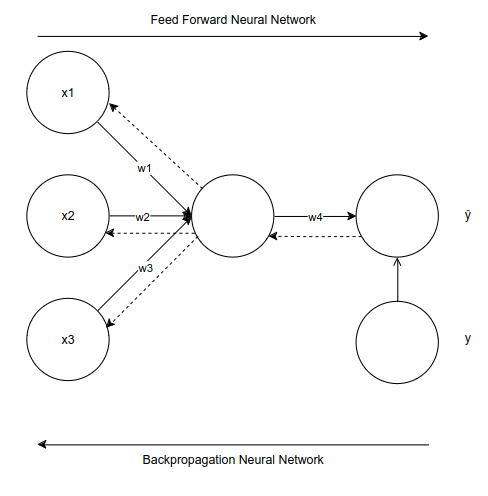
\includegraphics[scale=0.6]{gambar/bab2-ff-backprop.png}
  \caption{Perbedaan antara \emph{Feed Forward} dan \emph{Backpropagation}}
  \label{fig:ff_backprop}
\end{figure}

 \subsubsection{\emph{Loss Function} dan \emph{Optimizer}}
 \emph{Loss function} mengukur seberapa baik model NN melakukan prediksi dibandingkan dengan nilai sebenarnya. \emph{Loss function} yang umum meliputi:
 \begin{itemize}[nolistsep]
   \item \textbf{\emph{Gradient Descent}}: Metode optimisasi yang digunakan untuk meminimalkan fungsi kerugian dengan mengupdate bobot jaringan berdasarkan gradien fungsi kerugian.
   \item \textbf{\emph{Stochastic Gradient Descent} (SGD)}: Versi sederhana dari \emph{Gradient Descent} yang memperbarui bobot jaringan berdasarkan gradien dari satu sampel data.
   \item \textbf{\emph{Momentum}}: Metode optimisasi yang membantu percepatan konvergensi dengan menambahkan momentum pada proses \emph{Gradient Descent}.
   \item \textbf{\emph{RMSprop}}: Metode optimisasi yang menyesuaikan laju pembelajaran untuk setiap parameter berdasarkan gradien rata-rata kuadrat sebelumnya.
   \item \textbf{\emph{Adam}}: Algoritma optimisasi yang menggabungkan konsep dari \emph{Momentum} dan \emph{RMSprop} untuk memperbarui bobot jaringan secara adaptif.
 \end{itemize}
 
 Optimisasi adalah proses mencari parameter model yang meminimalkan fungsi kerugian. Algoritma optimisasi yang sering digunakan antara lain \emph{Stochastic Gradient Descent} (SGD), \emph{Adam}, dan \emph{RMSprop}. Adapun pada penelitian ini, digunakan algoritma Adam sebagai \emph{optimizer} untuk memperbarui bobot jaringan karena kemampuannya dalam menyesuaikan laju pembelajaran secara adaptif.
 
 \subsubsection{CNN (\emph{Convolutional Neural Network})}
 CNN (\emph{Convolutional Neural Networks}) memperluas konsep NN dengan memasukkan lapisan konvolusi, yang menggunakan filter untuk mengekstraksi fitur spatial dari data \emph{input}. Berikut merupakan beberapa konsep dasar dalam CNN:
 \begin{itemize}[nolistsep] 
   \item \textbf{\emph{Convolutional Layer}}: Menggunakan filter atau \emph{kernel} yang 'meluncur' di atas gambar untuk menghasilkan \emph{feature map}.
   \item \textbf{\emph{Stride}}: Jumlah piksel yang dilewati filter pada setiap gerakan. Stride yang lebih besar menghasilkan \emph{feature map} yang lebih kecil.
   \item \textbf{\emph{Padding}}: Penambahan piksel di sekitar input untuk memungkinkan filter beroperasi di tepi gambar.
   \item \textbf{\emph{Pooling Layer}} (\emph{Subsampling}): Mengurangi dimensi spatial dari \emph{feature map} untuk mengurangi jumlah parameter dan komputasi. Contohnya adalah \emph{max pooling} dan \emph{average pooling}.
   \item \textbf{\emph{Fully Connected Layer}}: Lapisan di mana setiap neuron terhubung ke semua neuron di lapisan sebelumnya, biasanya digunakan di akhir jaringan untuk mengklasifikasikan fitur yang diekstraksi oleh lapisan konvolusi.
 \end{itemize} 

 CNN merupakan salah satu arsitektur \emph{deep learning} yang paling banyak digunakan dalam pengolahan citra. CNN pertama kali diperkenalkan oleh Yan LeCun et al. \parencite*{yannlecun1998} dalam penelitian tentang pengenalan tulisan tangan menggunakan LeNet-5. Model ini menggabungkan operasi konvolusi, \emph{subsampling} (\emph{pooling}), dan \emph{fully connected layers} untuk mengekstraksi fitur secara hierarkis dari gambar \emph{input}.
 
Perkembangan CNN semakin pesat dengan adanya inovasi pada arsitektur. Salah satu inovasi signifikan adalah \emph{Residual Neural Network} (ResNet) yang diperkenalkan oleh Kaiming He et al. \parencite*{kaiminghe2015}. ResNet memperkenalkan konsep \emph{skip connection} yang memungkinkan model untuk belajar representasi yang lebih baik dari data. Hal ini memungkinkan model untuk dilatih dengan kedalaman yang lebih besar tanpa mengalami masalah \emph{vanishing gradient}.
 
Selain itu, metode modern seperti normalisasi \emph{batch} (\emph{BatchNorm}) yang dikembangkan oleh Ioffe et al. \parencite*{ioffe2015} dan Szegedy et al. \parencite*{szegedy2015} telah menjadi standar dalam \emph{training} CNN. \emph{BatchNorm} membantu jaringan untuk melakukan konvergensi lebih cepat dengan menormalkan distribusi setiap \emph{batch} selama pelatihan. Penggunaan konvolusi 1x1, seperti pada arsitektur \emph{Inception}, juga memperkenalkan cara baru untuk mengurangi jumlah parameter sambil mempertahankan kapasitas jaringan.
 
Penerapan CNN telah meluas ke berbagai domain, termasuk deteksi objek, segmentasi citra, dan pengenalan pola. Dalam konteks penelitian ini, CNN digunakan untuk mendeteksi kendaraan overdimensi berdasarkan karakteristik visualnya. Pendekatan ini sesuai dengan studi sebelumnya yang menunjukkan kemampuan CNN dalam mengolah data visual dengan tingkat akurasi yang tinggi.
\subsection{SSD (\emph{Single Shot MultiBox Detector})}

\emph{Single Shot MultiBox Detector} (SSD) adalah arsitektur deteksi objek yang dikembangkan oleh Liu et al. \parencite*{liu2016}. SSD memperkenalkan pendekatan \emph{single shot} yang memungkinkan model untuk melakukan deteksi objek dan klasifikasi dalam satu langkah. Hal ini berbeda dengan pendekatan \emph{two-stage} seperti Faster R-CNN yang memerlukan dua tahap untuk deteksi objek.

SSD menggunakan \emph{multi-scale feature maps} untuk mendeteksi objek pada berbagai skala. Arsitektur ini terdiri dari \emph{base network} (biasanya menggunakan arsitektur VGG16 atau ResNet) yang diikuti oleh beberapa lapisan konvolusi untuk menghasilkan \emph{feature maps} pada berbagai resolusi. Setiap lapisan \emph{feature map} digunakan untuk memprediksi \emph{bounding box} dan kelas objek yang terdapat dalam gambar.

\begin{figure}[H]
  \centering
  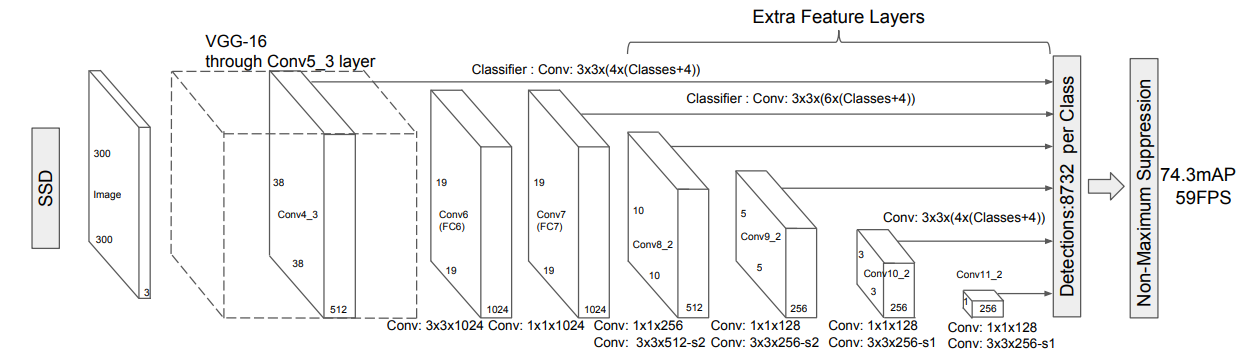
\includegraphics[scale=0.36]{gambar/bab2-arsitektur-ssd.png}
  \caption{Arsitektur SSD}
  \label{fig:arsitektur_ssd}
\end{figure}

SSD telah terbukti efektif dalam deteksi objek pada berbagai \emph{dataset}, termasuk PASCAL VOC dan COCO. Keunggulan utama SSD adalah kemampuannya untuk melakukan deteksi objek secara cepat dan akurat dalam satu langkah. Dalam penelitian ini, SSD digunakan sebagai model deteksi untuk mengidentifikasi kendaraan overdimensi pada video pengamatan jalan raya.

\subsection{\emph{Metrics} untuk Evaluasi Model}

Dalam evaluasi performa model deteksi objek, metrik seperti \emph{Precision}, \emph{Recall}, \emph{Average Precision (AP)}, dan \emph{Mean Average Precision (mAP)} digunakan untuk mengukur seberapa baik model dalam mengenali dan mengklasifikasikan objek dalam citra.

\subsubsection{\emph{Precision} dan \emph{Recall}}

\emph{Precision} mengukur proporsi prediksi positif yang benar dari semua prediksi positif yang dibuat oleh model, sedangkan \emph{Recall} mengukur proporsi deteksi yang benar dari seluruh objek yang seharusnya terdeteksi. \emph{Precision} dan \emph{Recall} dihitung dengan rumus berikut:

\begin{equation}
\mbox{Precision} = \frac{\mbox{TP}}{\mbox{TP} + \mbox{FP}}
\label{eq:precision}
\end{equation}

\begin{equation}
\mbox{Recall} = \frac{\mbox{TP}}{\mbox{TP} + \mbox{FN}}
\label{eq:recall}
\end{equation}

di mana TP (True Positive) adalah jumlah deteksi yang benar, FP (False Positive) adalah jumlah deteksi yang salah, dan FN (False Negative) adalah jumlah objek yang tidak terdeteksi \parencite*{padilla2020survey}.

\subsubsection{\emph{Average Precision} (AP)}

\emph{Average Precision (AP)} adalah metrik yang menggabungkan precision dan recall untuk satu kelas objek. AP dihitung sebagai area di bawah kurva \emph{Precision-Recall} (PR), yang dapat dihitung dengan pendekatan diskrit sebagai:

\begin{equation}
\mbox{AP} = \sum_{k=1}^{n} P(k) \Delta r(k)
\label{eq:AP}
\end{equation}

di mana $P(k)$ adalah \emph{precision} pada threshold ke-$k$, dan $\Delta r(k)$ adalah perubahan \emph{recall} antara \emph{threshold} ke-$(k-1)$ dan ke-$k$. Metrik ini memberikan pemahaman yang lebih dalam tentang performa deteksi terhadap satu kelas objek \parencite*{oksuz2018localization}.

\subsubsection{\emph{Mean Average Precision} (mAP)}

\emph{Mean Average Precision (mAP)} adalah rata-rata dari AP untuk semua kelas dalam dataset. mAP banyak digunakan dalam benchmark seperti PASCAL VOC dan COCO untuk mengevaluasi kinerja menyeluruh dari sistem deteksi objek. Persamaan mAP yaitu:

\begin{equation}
\mbox{mAP} = \frac{1}{N} \sum_{i=1}^{N} \mbox{AP}_i
\label{eq:mAP}
\end{equation}

di mana $N$ adalah jumlah kelas dan $\mbox{AP}_i$ adalah nilai \emph{Average Precision} untuk kelas ke-$i$ \parencite*{padilla2020survey, oksuz2018localization}.

\subsection{\emph{Inference Time} dan FPS (\emph{Frames Per Second})}

Dalam konteks sistem deteksi berbasis \emph{deep learning}, dua metrik utama yang sering digunakan untuk mengukur performa sistem adalah \emph{inference time} dan \emph{frames per second} (FPS). \emph{Inference time} merujuk pada waktu yang dibutuhkan oleh model untuk memproses satu data input (misalnya satu citra) hingga menghasilkan keluaran. Sebaliknya, FPS mengacu pada jumlah \emph{frame} yang dapat diproses oleh sistem dalam satu detik. Kedua metrik ini saling berkaitan secara matematis dan sering kali digunakan secara bergantian untuk menilai kecepatan sistem dalam konteks \emph{real-time}.

Secara umum, hubungan antara keduanya dapat dinyatakan sebagai:
\begin{equation}
  \mbox{FPS} = \frac{1}{\mbox{Waktu Inferensi}}
  \label{eq:fps_inference_time}
\end{equation}
Artinya, semakin kecil waktu inferensi, semakin banyak \emph{frame} yang dapat diproses dalam satu detik, sehingga nilai FPS menjadi lebih tinggi.

Menurut Han et al. \parencite*{Canziani2016An} dalam studinya mengenai analisis model jaringan saraf dalam untuk aplikasi praktis, ditemukan bahwa terdapat hubungan hiperbolik antara akurasi dan waktu inferensi, yang menunjukkan bahwa peningkatan akurasi model sering kali disertai dengan peningkatan waktu inferensi, dan akibatnya menurunkan nilai FPS. Oleh karena itu, terdapat \emph{trade-off} yang perlu dipertimbangkan antara kecepatan pemrosesan dan akurasi model dalam pengembangan sistem berbasis visi komputer \emph{real-time}, terutama untuk aplikasi pada perangkat terbatas atau \emph{edge device}.

Studi ini juga menegaskan pentingnya pemilihan arsitektur model yang tepat untuk mencapai keseimbangan antara efisiensi dan performa. Dalam aplikasi seperti sistem \emph{real-time} atau deteksi objek bergerak, nilai FPS yang tinggi sangat diperlukan agar sistem dapat merespons secara tepat waktu terhadap perubahan lingkungan visual secara dinamis.

\subsection{\emph{Edge Computing}}

\emph{Edge computing} adalah paradigma komputasi yang memungkinkan pemrosesan data dilakukan di dekat sumber data, seperti perangkat \emph{IoT} (\emph{Internet of Things}) atau sensor. Hal ini bertentangan dengan komputasi tradisional yang memerlukan pengiriman data ke pusat data atau cloud untuk diproses. \emph{Edge computing} memungkinkan pemrosesan data yang lebih cepat, responsif, dan efisien dengan memanfaatkan sumber daya lokal.

Keuntungan utama dari \emph{edge computing} adalah kemampuannya untuk mengurangi latensi dan mempercepat respons sistem \parencite*{aws2024}. Dengan melakukan pemrosesan data di dekat sumber data, \emph{edge computing} memungkinkan aplikasi untuk merespons lebih cepat terhadap perubahan kondisi lingkungan. Hal ini sangat penting dalam konteks aplikasi \emph{real-time} seperti deteksi objek pada video pengamatan jalan raya.

Selain itu, \emph{edge computing} juga membantu mengurangi beban jaringan dan \emph{cloud} dengan melakukan pemrosesan data secara lokal. Hal ini dapat mengurangi biaya operasional dan meningkatkan efisiensi sistem secara keseluruhan. Dalam konteks penelitian ini, \emph{edge computing} digunakan untuk menjalankan model deteksi objek secara \emph{real-time} pada perangkat lokal tanpa memerlukan koneksi internet. 

Contoh implementasi \emph{edge computing} yang digunakan dalam penelitian ini adalah Jetson Nano dan Beelink Gemini T34 yang berfungsi sebagai \emph{edge device} untuk menjalankan model deteksi objek secara \emph{real-time}.

\subsubsection{Jetson Nano}

 \begin{figure}[htbp]
  \centering
  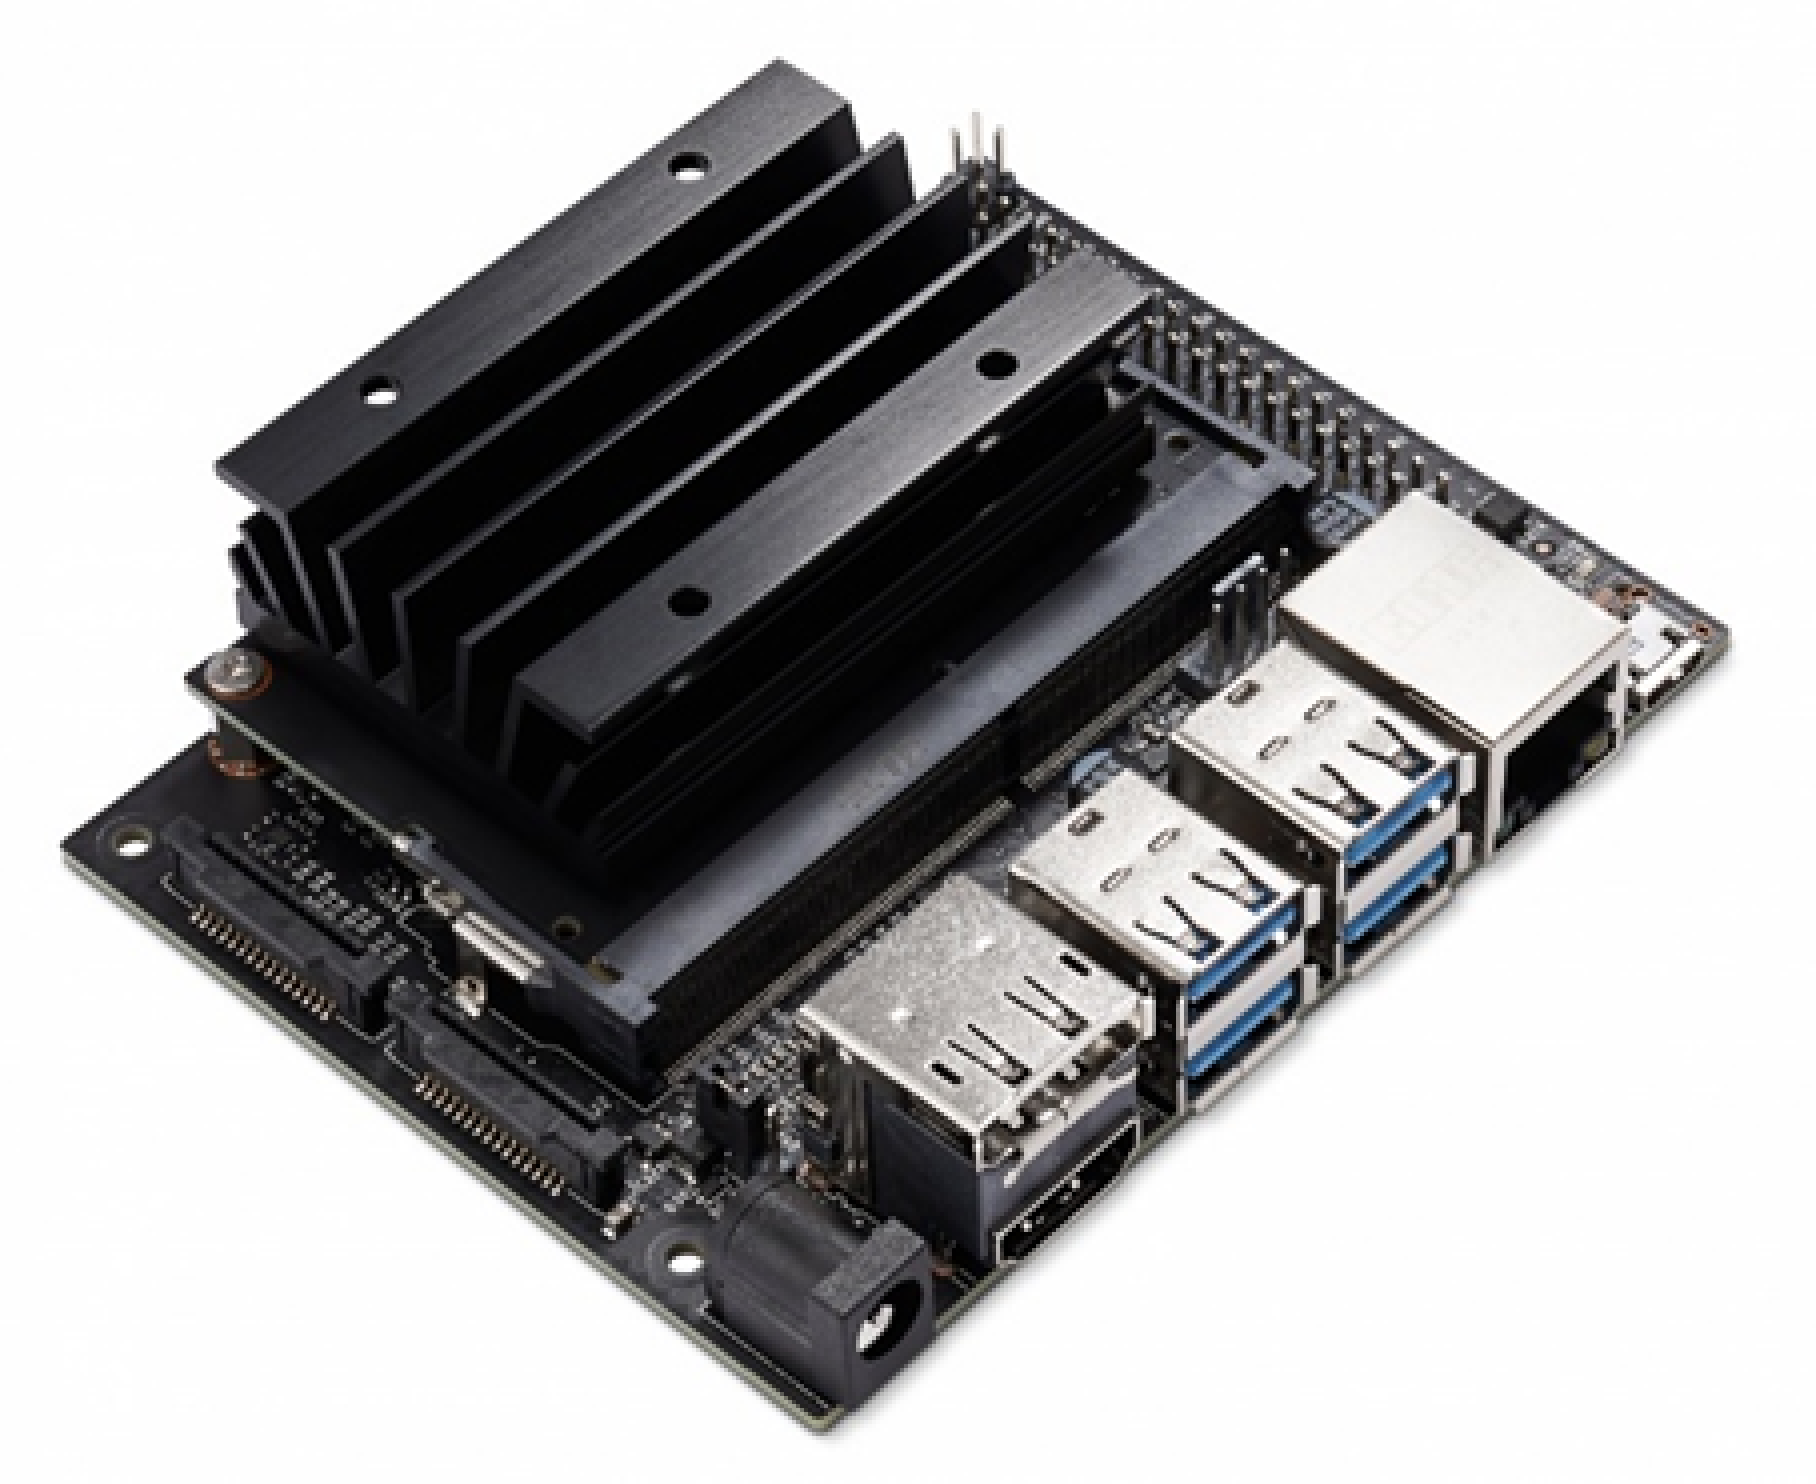
\includegraphics[scale=0.5]{gambar/bab2-jetson-nano.png}
  \caption{Jetson Nano Developer Kit}
  \label{fig:jetsonnano}
\end{figure}

Jetson Nano adalah perangkat komputasi keluaran NVIDIA yang didedikasikan dalam pengembangan \textit{machine learning} dan \emph{edge computing}. Jetson Nano memiliki kemampuan untuk dapat menjalankan beberapa \emph{neural networks} secara paralel. Kemampuan ini memungkinkan Jetson Nano untuk digunakan dalam \textit{image classification}, \textit{object detection}, \textit{segmentation}, dan \textit{speech processing} \parencite{nvidiaJetsonNano}. Perangkat ini dapat menjadi solusi dalam menjalankan model \textit{machine learning} atau \textit{deep learning} pada perangkat portable dan hemat energi. 

Perangkat ini dilengkapi dengan 128 NVIDIA CUDA \emph{cores}. Ditenagai oleh prosesor \emph{Quad-core ARM Cortex-A57 MPCore}, \emph{platform} ini menyediakan fungsionalitas komputasi yang solid dengan memori 4 GB 64-bit LPDDR4 yang beroperasi pada 1600MHz, memberikan \emph{bandwidth} 25.6 GB/s. Untuk penyimpanan, Jetson Nano dilengkapi dengan 16 GB eMMC 5.1, yang memberikan ruang yang cukup untuk aplikasi dan data pengguna. Jetson Nano dapat mengkodekan video dengan kecepatan 250MP/sec, mendukung format seperti 1x 4K pada 30fps (HEVC), 2x 1080p pada 60fps (HEVC), dan sebagainya. Sementara itu, untuk \emph{decode} video, perangkat ini menawarkan kemampuan hingga 500MP/sec, dengan dukungan untuk format seperti 1x 4K pada 60fps (HEVC) dan 2x 4K pada 30fps (HEVC). Jetson Nano juga dilengkapi dengan 12 jalur kamera (3x4 atau 4x2) MIPI CSI-2 D-PHY 1.1, yang mendukung kecepatan hingga 1.5 Gb/s per pasangan, memberikan fleksibilitas dalam pengembangan aplikasi berbasis kamera. Dalam hal konektivitas, perangkat ini menawarkan Gigabit Ethernet dan M.2 Key E, serta kemampuan tampilan melalui HDMI 2.0 dan eDP 1.4. Jetson Nano juga dilengkapi dengan 4x USB 3.0 dan USB 2.0 Micro-B, serta berbagai opsi konektivitas lainnya seperti GPIO, I2C, I2S, SPI, dan UART, semuanya dalam \emph{form factor} mekanis 69.6 mm x 45 mm dengan konektor tepi 260-pin \parencite{nvidiaJetsonNano}.

\subsubsection{Beelink Gemini T34}
 \begin{figure}[htbp]
     \centering
     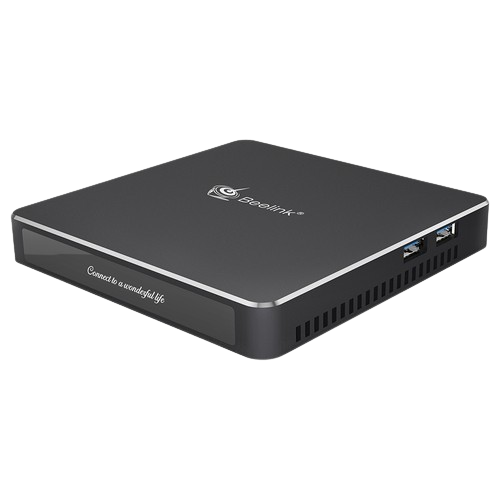
\includegraphics[scale=0.5]{gambar/bab2-beelink-gemini-t34.png}
     \caption{Beelink Gemini T34}
     \label{fig:beelinkgeminit34}
\end{figure}

Beelink Gemini T34 adalah mini PC yang dilengkapi dengan prosesor Intel Apollo Lake N3450. Prosesor ini memiliki 4 \emph{core} dan 4 \emph{thread} dengan kecepatan hingga 2.2 GHz. Beelink Gemini T34 juga dilengkapi dengan Intel HD Graphics 500 yang mendukung resolusi hingga 4K. Mini PC ini memiliki RAM 8 GB LPDDR3 dan penyimpanan 128 GB eMMC SSD. Beelink Gemini T34 memiliki berbagai port konektivitas seperti HDMI, USB 3.0, USB 2.0, dan Gigabit Ethernet. Mini PC ini juga dilengkapi dengan konektivitas Wi-Fi 5 dan Bluetooth 4.0. Beelink Gemini T34 memiliki dimensi 11.9 cm x 11.9 cm x 1.79 cm dan berat 0.4 kg, sehingga mudah dipindahkan dan ditempatkan di berbagai lokasi. \parencite*{beelinkGeminiT34}

Beelink Gemini T34 dapat digunakan sebagai \emph{edge device} untuk menjalankan model deteksi objek secara \emph{real-time}. Mini PC ini memiliki performa yang cukup untuk menjalankan aplikasi deteksi objek dengan akurasi tinggi dan latensi rendah. Dengan konektivitas Wi-Fi dan Bluetooth, Beelink Gemini T34 dapat terhubung ke jaringan lokal dan perangkat lain untuk mentransfer data deteksi objek.

\begin{table}[htbp]
  \centering
  \caption{Perbandingan Spesifikasi Jetson Nano dan Beelink Gemini T34}
  \label{tab:perbandingan_edge_device}
  \begin{tabular}{|p{3cm}|p{5cm}|p{5cm}|}
    \hline
    \textbf{Spesifikasi} & \textbf{Jetson Nano} & \textbf{Beelink Gemini T34} \\
    \hline
    Prosesor & Quad-core ARM Cortex-A57 MPCore & Intel Apollo Lake N3450 (4 core, 4 thread) \\
    \hline
    GPU & 128 NVIDIA CUDA \emph{cores} & Intel HD Graphics 500 \\
    \hline
    RAM & 4 GB 64-bit LPDDR4 (25.6 GB/s) & 8 GB LPDDR3 \\
    \hline
    Penyimpanan & 16 GB eMMC 5.1 & 128 GB eMMC SSD \\
    \hline
    Kemampuan Video & \begin{itemize}[nolistsep]
      \item \emph{Encode}: 250MP/sec
      \item \emph{Decode}: 500MP/sec
      \item 4K @ 30fps (HEVC)
    \end{itemize} & \begin{itemize}[nolistsep]
      \item Mendukung resolusi 4K
      \item Hardware decoding
    \end{itemize} \\
    \hline
    Konektivitas & \begin{itemize}[nolistsep]
      \item Gigabit Ethernet
      \item 4x USB 3.0
      \item HDMI 2.0
      \item GPIO, I2C, I2S, SPI
    \end{itemize} & \begin{itemize}[nolistsep]
      \item Gigabit Ethernet
      \item USB 3.0, USB 2.0
      \item HDMI
      \item Wi-Fi 5
      \item Bluetooth 4.0
    \end{itemize} \\
    \hline
    Dimensi & 69.6 mm x 45 mm & 119 mm x 119 mm x 17.9 mm \\
    \hline
    Keunggulan untuk AI & \begin{itemize}[nolistsep]
      \item CUDA \emph{cores} untuk akselerasi AI
      \item Optimasi untuk \emph{deep learning}
      \item Dukungan \emph{framework} AI
    \end{itemize} & \begin{itemize}[nolistsep]
      \item CPU x86 standar
      \item Kompatibilitas \emph{software} lebih luas
      \item Penyimpanan lebih besar
    \end{itemize} \\
    \hline
  \end{tabular}
\end{table}

Kedua perangkat memiliki keunggulan masing-masing sebagai \emph{edge device}. Jetson Nano unggul dalam kemampuan pemrosesan AI berkat CUDA \emph{cores}-nya, sementara Beelink Gemini T34 menawarkan fleksibilitas lebih tinggi dengan arsitektur x86 dan penyimpanan yang lebih besar. Pemilihan antara keduanya dapat disesuaikan dengan kebutuhan spesifik implementasi sistem.

\subsection{\emph{Quality of Service}}

Kualitas Layanan atau \emph{Quality of Service} (QoS) didefinisikan sebagai suatu mekanisme pada jaringan komputer yang memungkinkan penyediaan layanan yang berbeda untuk kelas-kelas aplikasi yang berbeda pula. Dalam konteks jaringan internet, QoS merujuk pada kemampuan jaringan untuk menyediakan layanan yang lebih baik untuk trafik tertentu dibandingkan dengan trafik lainnya. Tujuan utama dari implementasi QoS adalah untuk mencapai tingkat performa jaringan yang dapat diprediksi dan dijamin, terutama untuk aplikasi-aplikasi yang sensitif terhadap kualitas jaringan seperti \emph{streaming video}, \emph{voice over IP} (VoIP), dan \emph{online gaming}.

Parameter-parameter yang umum digunakan untuk mengukur QoS, sebagaimana disebutkan sebelumnya, meliputi:

\begin{itemize}
    \item \textbf{\emph{Throughput}}: Mengacu pada laju transfer data efektif yang berhasil dikirimkan melalui suatu jalur komunikasi dalam satuan waktu tertentu, biasanya diukur dalam bit per detik (bps) atau kelipatannya (kbps, Mbps). Persamaan \ref{eq:throughput} digunakan untuk menghitung \emph{throughput}.
    \begin{equation}
      \label{eq:throughput}
      \mbox{Throughput} = \frac{\mbox{Jumlah Data yang dikirim}}{\mbox{Waktu pengiriman data}}
    \end{equation}
    \item \textbf{\emph{Packet Loss}}: Merupakan persentase paket data yang hilang atau gagal mencapai tujuan selama proses transmisi. Kehilangan paket dapat disebabkan oleh berbagai faktor seperti kongesti jaringan, \emph{error} pada media transmisi, atau \emph{buffer overflow} pada perangkat jaringan. Persamaan \ref{eq:packetloss} digunakan untuk menghitung \emph{packet loss}.
    \begin{equation}
      \label{eq:packetloss}
      \mbox{Packet Loss} = \frac{\mbox{(Paket data dikirim - Paket data diterima)}}{\mbox{Paket data dikirim} * 100\%}
    \end{equation}
    \item \textbf{\emph{Delay (Latency)}}: Adalah total waktu yang dibutuhkan oleh sebuah paket data untuk menempuh perjalanan dari titik asal ke titik tujuan. \emph{Delay} terdiri dari beberapa komponen, termasuk \emph{\emph{propagation delay}}, \emph{\emph{transmission delay}}, \emph{\emph{processing delay}}, dan \emph{\emph{queuing delay}}. Persamaan \ref{eq:delay} digunakan untuk menghitung \emph{delay}.
    \begin{equation}
      \label{eq:delay}
      \mbox{Delay} = \frac{\mbox{Total paket delay}}{\mbox{Total paket yang diterima}}
    \end{equation}
    \item \textbf{\emph{Jitter}}: Didefinisikan sebagai variasi atau fluktuasi dalam \emph{delay} antar paket yang diterima secara berurutan. \emph{Jitter} yang tinggi dapat berdampak negatif pada kualitas aplikasi \emph{real-time} seperti audio dan video. Persamaan \ref{eq:jitter} digunakan untuk menghitung \emph{jitter}.
    \begin{equation}
      \label{eq:jitter}
      \mbox{Jitter} = \frac{\mbox{Total variasi delay}}{\mbox{Total paket yang diterima}}
    \end{equation}
    dimana untuk mencari total variasi \emph{delay}, dapat menggunakan persamaan \ref{eq:totalvariasidelay}:
    \begin{equation}
      \label{eq:totalvariasidelay}
      \mbox{Total variasi delay} = \sum_{i=1}^{n-1} (D_{i+1} - D_i)
    \end{equation}
\end{itemize}

Pentingnya pengukuran \emph{QoS}, terutama pada jaringan nirkabel seperti WiFi, ditekankan karena sifat medium transmisinya yang lebih rentan terhadap gangguan. Faktor-faktor eksternal seperti kondisi cuaca, interferensi dari gelombang elektromagnetik lain, serta halangan fisik dapat secara signifikan mempengaruhi stabilitas dan kualitas transmisi data pada jaringan WiFi, yang pada gilirannya akan berdampak pada parameter-parameter \emph{QoS}. Oleh karena itu, pemantauan dan pengelolaan \emph{QoS} menjadi krusial untuk memastikan pengalaman pengguna yang optimal pada berbagai jenis layanan jaringan. \parencite*{hariesanom2024}

\subsection{RESTful API}

RESTful API (\emph{Representational State Transfer Application Programming Interface}) adalah arsitektur desain yang digunakan untuk membangun layanan web yang ringan, fleksibel, dan mudah diakses. RESTful API menggunakan prinsip REST yang memisahkan antara data dan tampilan, serta memanfaatkan metode HTTP untuk berkomunikasi antara klien dan server.

RESTful API menggunakan 4 metode HTTP utama untuk berinteraksi dengan \emph{resource}:
\begin{itemize}[nolistsep]
  \item \textbf{GET}: Mengambil data dari \emph{resource}.
  \item \textbf{POST}: Membuat data baru di \emph{resource}.
  \item \textbf{PUT}: Memperbarui data yang ada di \emph{resource}.
  \item \textbf{DELETE}: Menghapus data dari \emph{resource}.
\end{itemize}

RESTful API menggunakan URI (\emph{Uniform Resource Identifier}) untuk mengidentifikasi sumber daya yang diakses dan format data yang diinginkan. Data dikirimkan dalam format yang umum seperti JSON atau XML untuk memudahkan pertukaran data antara klien dan server. \parencite*{restapi2016}

Keunggulan utama dari RESTful API adalah kemudahan penggunaan, fleksibilitas, dan skalabilitas. RESTful API memungkinkan pengembang untuk membangun layanan \emph{web} yang dapat diakses dari berbagai \emph{platform} dan bahasa pemrograman. Dalam penelitian ini, RESTful API digunakan untuk mengintegrasikan antara aplikasi Flutter dengan \emph{cloud} untuk mentransfer data deteksi objek secara \emph{real-time}.

\subsection{Flutter}

Flutter adalah \emph{framework} pengembangan aplikasi \emph{open-source} yang dikembangkan oleh \emph{Google} \parencite*{google2024}. Flutter memungkinkan pengembang untuk membuat aplikasi \emph{mobile} dengan antarmuka pengguna yang kaya dan responsif. Flutter menggunakan bahasa pemrograman Dart yang dikembangkan oleh Google sebagai bahasa utamanya.

Keunggulan utama dari Flutter adalah kemampuannya untuk membuat aplikasi \emph{mobile} yang konsisten di berbagai \emph{platform}, termasuk Android dan iOS. Flutter menggunakan \emph{widget} sebagai komponen dasar untuk membangun antarmuka pengguna. \emph{Widget} Flutter bersifat deklaratif, yang berarti pengembang mendefinisikan bagaimana antarmuka pengguna harus terlihat berdasarkan kondisi saat ini.

Flutter juga menyediakan berbagai \emph{plugin} dan \emph{package} yang memperluas fungsionalitas aplikasi. Pengembang dapat menggunakan \emph{plugin} Flutter untuk mengakses fitur perangkat seperti kamera, lokasi, dan sensor. Selain itu, Flutter juga menyediakan \emph{package} untuk mengintegrasikan aplikasi dengan layanan \emph{cloud}, \emph{database}, dan API eksternal.

Dalam penelitian ini, Flutter digunakan sebagai \emph{platform} pengembangan aplikasi \emph{mobile} untuk menampilkan hasil deteksi objek secara \emph{real-time}. Aplikasi Flutter akan berkomunikasi dengan \emph{cloud} untuk menerima data deteksi objek dan menampilkannya dalam antarmuka pengguna yang responsif.

\subsection{PostgreSQL}

PostgreSQL adalah sistem manajemen basis data relasional (\emph{RDBMS}) yang bersifat \emph{open-source} dan dapat diandalkan. PostgreSQL dikembangkan oleh komunitas pengembang yang aktif dan memiliki fitur yang lengkap untuk mengelola data dalam skala besar. PostgreSQL menggunakan bahasa SQL (\emph{Structured Query Language}) untuk berinteraksi dengan basis data dan mendukung berbagai jenis data dan operasi. \parencite*{postgresql2025}

Keunggulan utama dari PostgreSQL adalah keandalan, fleksibilitas, dan skalabilitas. PostgreSQL memiliki fitur transaksi ACID (\emph{Atomicity, Consistency, Isolation, Durability}) yang memastikan konsistensi data dan keandalan operasi. PostgreSQL juga mendukung berbagai jenis data seperti teks, angka, geometri, dan JSON, serta operasi kompleks seperti \emph{join}, \emph{subquery}, dan \emph{trigger}.

PostgreSQL juga memiliki dukungan yang baik untuk pengelolaan data dalam skala besar. PostgreSQL mendukung indeks, partisi, dan \emph{replication} untuk meningkatkan kinerja dan ketersediaan sistem. Selain itu, PostgreSQL juga memiliki fitur keamanan yang kuat seperti autentikasi, otorisasi, dan enkripsi data.

Dalam penelitian ini, PostgreSQL digunakan sebagai basis data untuk menyimpan data deteksi objek dan data pengguna. PostgreSQL akan digunakan untuk menyimpan informasi tentang objek yang terdeteksi, lokasi deteksi, dan waktu deteksi. Basis data ini akan digunakan oleh aplikasi Flutter untuk menampilkan data deteksi objek dan memungkinkan pengguna untuk melihat riwayat deteksi objek.

\subsection{Express.js}

Express.js adalah kerangka kerja web \emph{back-end} untuk Node.js yang minimalis dan fleksibel. Express.js menyediakan serangkaian fitur untuk membangun aplikasi web dan API dengan cepat dan mudah. Express.js menggunakan pendekatan \emph{middleware} yang memungkinkan pengembang untuk menambahkan fungsionalitas secara modular ke dalam aplikasi. \parencite*{expressjs2024}

Keunggulan utama Express.js meliputi:
\begin{itemize}[nolistsep]
  \item \textbf{Minimalis dan Fleksibel}: Express.js menyediakan fitur dasar yang diperlukan untuk membangun aplikasi web tanpa memaksakan struktur atau konvensi tertentu.
  \item \textbf{\emph{Middleware}}: Sistem \emph{middleware} memungkinkan pengembang untuk menambahkan fungsionalitas seperti \emph{logging}, autentikasi, dan penanganan kesalahan secara modular.
  \item \textbf{\emph{Routing}}: Express.js menyediakan sistem \emph{routing} yang kuat untuk menangani permintaan HTTP dengan berbagai metode dan parameter.
  \item \textbf{\emph{Template Engine}}: Mendukung berbagai \emph{template engine} untuk menghasilkan tampilan HTML dinamis.
\end{itemize}

\subsection{Apache HTTP Server}

Apache HTTP Server (Apache2) adalah server web \emph{open-source} yang paling banyak digunakan di dunia. Apache2 dikembangkan dan dikelola oleh Apache Software Foundation dan mendukung berbagai \emph{platform} sistem operasi. Server ini dikenal karena kehandalannya, fleksibilitas konfigurasi, dan ekosistem modul yang luas. \parencite*{apache2024}

Fitur utama Apache2 meliputi:
\begin{itemize}[nolistsep]
  \item \textbf{\emph{Virtual Hosting}}: Kemampuan untuk menjalankan beberapa situs \emph{web} pada satu \emph{server}.
  \item \textbf{Modul Dinamis}: Mendukung penambahan dan penghapusan modul tanpa mengompilasi ulang \emph{server}.
  \item \textbf{Keamanan}: Menyediakan fitur keamanan seperti SSL/TLS, autentikasi, dan otorisasi.
  \item \textbf{\emph{Reverse Proxy}}: Dapat berfungsi sebagai \emph{reverse proxy} untuk mendistribusikan beban dan meningkatkan keamanan.
\end{itemize}

Dalam penelitian ini, Apache2 digunakan sebagai \emph{server} untuk menjalankan aplikasi \emph{backend}. Apache2 akan memastikan bahwa aplikasi \emph{backend} dapat diakses publik dan siap menangani permintaan dari aplikasi Flutter.

\subsection{PM2 (Process Manager 2)}

PM2 adalah manajer proses untuk aplikasi Node.js yang memungkinkan pengembang untuk mengelola dan mempertahankan aplikasi tetap berjalan di lingkungan produksi. PM2 menyediakan fitur-fitur penting seperti \emph{load balancing}, \emph{monitoring}, dan manajemen log untuk memastikan ketersediaan dan kinerja aplikasi. \parencite*{pm22024}

Keunggulan utama PM2 meliputi:
\begin{itemize}[nolistsep]
  \item \textbf{\emph{Process Management}}: Kemampuan untuk menjalankan aplikasi dalam mode \emph{daemon}, \emph{restart} otomatis saat \emph{crash}, dan \emph{update} tanpa \emph{downtime}.
  \item \textbf{\emph{Load Balancing}}: Mendistribusikan beban di antara beberapa instance aplikasi untuk meningkatkan \emph{throughput}.
  \item \textbf{\emph{Monitoring}}: Menyediakan dashboard untuk memantau penggunaan \emph{CPU}, \emph{memory}, dan metrik lainnya secara \emph{real-time}.
  \item \textbf{\emph{Log Management}}: Mengelola dan merotasi file log untuk mencegah penggunaan disk yang berlebihan.
\end{itemize}

Dalam penelitian ini, PM2 digunakan untuk mengelola dan mempertahankan aplikasi \emph{backend} agar tetap berjalan di lingkungan produksi. PM2 akan memastikan bahwa aplikasi \emph{backend} tetap berjalan dan siap menangani permintaan dari aplikasi Flutter.

\subsection{Cloudinary}

Cloudinary adalah layanan \emph{cloud-based} untuk menyimpan, mengelola, dan mengirim media digital. Cloudinary menyediakan fitur-fitur untuk memudahkan pengembang dalam mengelola media digital seperti gambar, video, dan dokumen. \parencite*{cloudinary2024}

Keunggulan utama Cloudinary meliputi:
\begin{itemize}[nolistsep]
  \item \textbf{\emph{Storage}}: Menyediakan penyimpanan media digital yang aman dan skalabel.
  \item \textbf{\emph{Transformation}}: Menyediakan fitur untuk memanipulasi media digital seperti crop, resize, dan filter.
  \item \textbf{\emph{Delivery}}: Menyediakan fitur untuk mengirim media digital ke berbagai \emph{platform} dan \emph{device}.
\end{itemize}

Dalam penelitian ini, Cloudinary digunakan untuk menyimpan dan mengirim gambar deteksi objek. Cloudinary akan memastikan bahwa gambar deteksi objek dapat disimpan tautannya di basis data PostgreSQL.